\chapter{Evaluation}

\section{Customer Requirements}

For this section I will be evaluating whether or not my system has met my initial objectives that were proposed in the Analysis section. This will be used to determine whether or not the system has met the customer requirements. If the system does not meet an objective then I will include a further explanation of why this is the case. If the objective has been met then I will provide evidence to support this evaluation.

The objectives have been split into:
\begin{itemize}
\item{General Objectives}
\item{Specific Objectives}
\item{Core Objectives}
\item{Other Objectives}
\end{itemize}

%include as many subsections as necessary for your objectives
\paragraph{General Objectives}

\subsection{Database Functionality}

\textbf{Objective:} A database to show all current staff (with details such as their job title) and the hardware devices they are assigned to.

\textbf{Has the objective been fulfilled?}

This objective has been fulfilled. I have met this objective by examining the company's current spreadsheet (their current way to store data) and making sure that all the correct fields were included in my database. To display allocation of hardware devices to staff members it was important to make the database relational, this was done with the use of primary and foreign keys. Using this method means hardware can be added to a separate table to staff and then linked in the StaffHardware table which the staff members will see.

\textbf{Evidence}

Below are the different interfaces that will present the database that shows current staff and their assigned hardware devices.

\begin{figure}[H]
    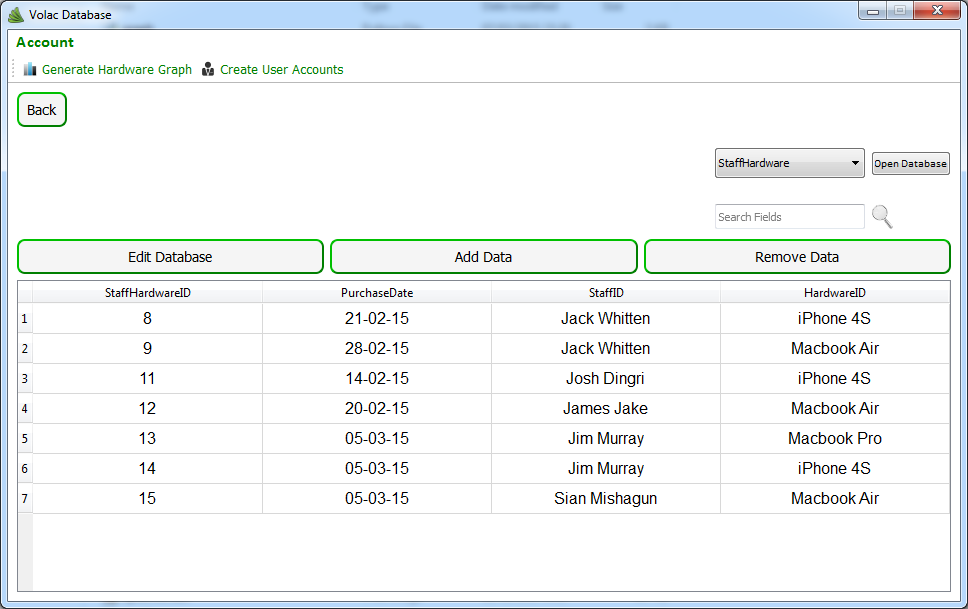
\includegraphics[width=\textwidth]{./Evaluation/Images/Database1.png}
    \caption{The Admin interface, viewing the StaffHardware Table.} \label{fig:db1}
\end{figure}

\begin{figure}[H]
    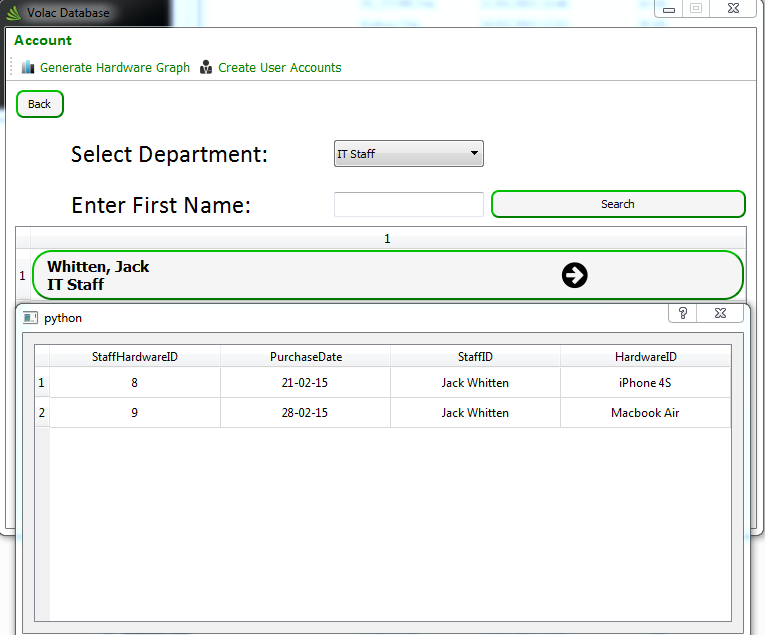
\includegraphics[width=\textwidth]{./Evaluation/Images/database3.png}
    \caption{The Admin interface: When searching for data and clicking to view more information, the StaffHardware table will appear.} \label{fig:db2}
\end{figure}

\begin{figure}[H]
    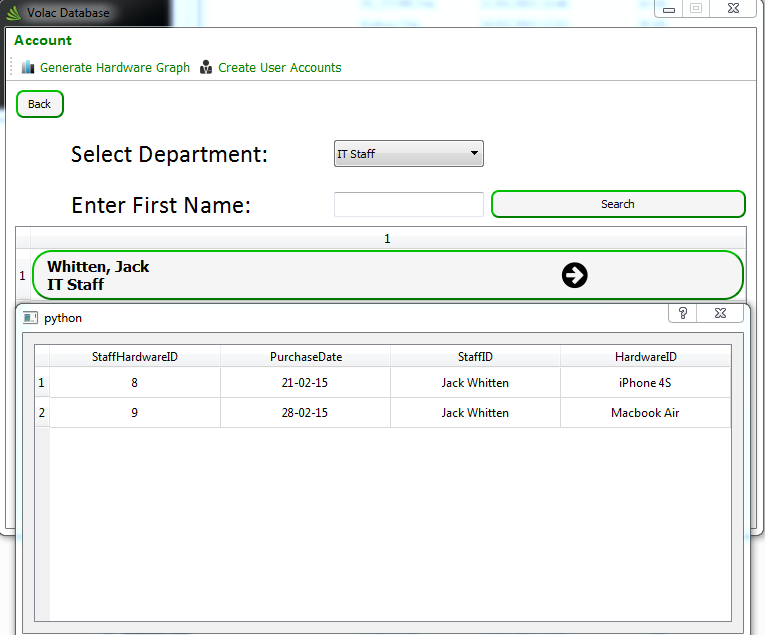
\includegraphics[width=\textwidth]{./Evaluation/Images/database3.png}
    \caption{The Manager (and staff) interface, viewing their current hardware devices.} \label{fig:db3}
\end{figure}

\subsection{Clear Database Structure}

\textbf{Objective:} The database will replace the current spreadsheet and be easy to read as information will be clear and organized.

\textbf{Has the objective been fulfilled?}

The objective has been met. The database includes all the needed fields from the spreadsheet and makes use of drop down boxes to make data organised. Each table is viewed by selecting it from the drop down box which means there is not too much information on the screen at one time. The font size was increased so the data is easy to read and the system has been spaced out so information is not cluttered.

\textbf{Evidence}


\subsection{Easy to use Data Input and Keyboard Shortcuts}

\textbf{Objective:} An easy to use database for IT staff to enter colleague data with toolbar buttons and keyboard shortcuts as they are advanced computer users and will want an quicker way of doing things.

\textbf{Has the objective been fulfilled?}

The objective has been fulfilled. There are toolbar buttons on the admin interface to allow account and graph generations. There are also keyboard shortcuts that are linked to some of the menubar buttons so staff can use them quickly, for example using F1 and F2 (for managers) to switch between layouts. Some of the shortcuts suggested in the design have been left out, the user will not be able to choose a table to edit from the menubar. 

\textbf{Evidence}


\subsection{Simple Interface Structure}

\textbf{Objective:} The layout for colleagues to see their hardware allocations will be clear and to the point, missing out any unnecessary buttons and menus.

\textbf{Has the objective been fulfilled?}

The objective has been fulfilled. I have ensured that there is not too many buttons on the system and that all buttons are clearly labeled. I did not include a menu from the design because it was unnecessary. For the staff interface they have a simply table showing their devices  since they do not need any extra features. 

\textbf{Evidence}


\subsection{Search Functionality}\label{search}

\textbf{Objective:} A search function will be in place to make searching for a field (such as staff member or hardware device) easy.

\textbf{Has the objective been fulfilled?}

The objective has been fulfilled. There are search functions on every interface which enables staff to easily search the table. The admin interface also has a more advanced search which allows them to search for staff members by department and then click to view more information about their colleague. The basic search function on each table allows users to search for any field in the table, simply by entering text into the search box the table will automatically search for the data.

\textbf{Evidence}



%%%%
\paragraph{Specific Objectives}

\subsection{Tables}

\textbf{Objective:}The database will have one table with staff and a relationship to the table with their hardware device. This will show which hardware devices the staff are allocated and all the details of that hardware device. Staff details including department and location will be linked to the Department and Location tables.

\textbf{Has the objective been fulfilled?}

The objective has been met. All relationships have been made successfully which reduces data duplication and some fields can be chosen simply by selecting from drop down boxes. The StaffHardware table (linking staff with hardware devices) is present on each interface since this is the most important and main table for viewing allocated hardware devices.

\textbf{Evidence}



\subsection{How the System will Search for Data}

\textbf{Objective:}The search function will allow a user to enter text and will highlight where on the page that text is.

\textbf{Has the objective been fulfilled?}

This specific objective has not been met, but has instead been improved. The reason for this is that I have changed how the search function works. It was not efficient to have to data be highlighted when the user enters text because if there was a lot of data it would still be hard to find the highlighted text. I have changed this so the table only shows the data that meets the search criteria, all other records will be hidden. For example if the user was to search for "Financing" all the staff members from the Financing department would be shown.

\textbf{Evidence}


\subsection{Read-Only access for staff}

\textbf{Objective:} Read-Only access for staff viewing their own information (with a log-in system to allow this).

\textbf{Has the objective been fulfilled?}

This objective has been met. The lowest access level (for normal staff use) displays the "StaffHardware" table in read only format, which means no data can be modified. The login system allows the staff to log in to their interface, each interface has its own access restrictions. In order of how much access received, the interfaces are Admin, Manager and Staff.

\textbf{Evidence}



\subsection{Read-Only access for managers}

\textbf{Objective:}Read-Only access for line managers wanting to see all data about staff in their department.

\textbf{Has the objective been fulfilled?}

This objective has been fulfilled. Managers have read only access to the table which displays information about their department.

\textbf{Evidence}



\subsection{Admin access for IT Staff}

\textbf{Objective:}Admin rights for IT staff so they are able to view and edit all data on the database.

\textbf{Has the objective been fulfilled?}

Objective has been fulfilled. Admin access allow the user to  view all of the tables in the database in order to add, edit and remove any data. When creating log in accounts, the user can give admin access to any staff member, so when the company come to use the system it may not be just IT Staff as the objective says.

\textbf{Evidence}



\subsection{Querying Data}

\textbf{Objective:} Users will be able to query information, for example if they wanted to show only mobile phones or if they wanted to show only specific departments.

\textbf{Has the objective been fulfilled?}

The objective has been met by using the search functions on each table but there is no advanced way to query data, apart from using the admin interface to search for staff by department. (Referenced also in section \ref{search})

\textbf{Evidence}



\paragraph{Core Objectives}

\subsection{The Login System}

\textbf{Objective:}The system will provide a login system where IT staff can assign usernames to all staff and have admin rights to view all data. The database will have read-only access for colleagues viewing their own information. Managers will be able to view their departments hardware devices.

\textbf{Has the objective been fulfilled?}

Objective has been fulfilled. IT Staff (or admins) can successfully create usernames and password for other staff members that they can then use to log in to the system with. Admins can also view all tables in the database and add, edit and remove data. Managers can log in the their interface where they can view their departments data along with their own hardware devices. Other staff can log in to the basic interface that will allow them to view their own data.

\textbf{Evidence}



\subsection{Automatic Email}

\textbf{Objective:}The system will also have an automatic email sent to IT staff members reminding them that a warranty is running out on a particular device, this email will be sent about 3 months before the end of the warranty period.

\textbf{Has the objective been fulfilled?}

The objective has been fulfilled. When the system has been started it will check to see if any hardware warranties  are set to expire in 90 days (rounded from 3 months). If a device is going to expire an email will be sent to the email set in the system (which will be the IT Staff email). The automatic email does not work as efficiently has it could because it will not automatically work out dates while the program is running, instead it can only work out the days left if the program is restarted once a day. However most likely the program would be reset each day in a real company, but it is still a big problem that would need to be fixed at a later date.

\textbf{Evidence}



\subsection{Search Function}

\textbf{Objective:}The system must have a search function to allow a user to find a specific field.

\textbf{Has the objective been fulfilled?}

Objective has been fulfilled. 

\textbf{Evidence}



\subsection{--}

\textbf{Objective:}The system must have a way to query information so that a user can filter or catergorise information (such as by department or location)

\textbf{Has the objective been fulfilled?}

\textbf{Evidence}


\paragraph{Other Objectives}

\subsection{--}

\textbf{Objective:}It will be nice to include a method of sending hardware request forms electronically to elimate the need for physical copies. However this will only be considered if everything else is completed as it is not essential.

\textbf{Has the objective been fulfilled?}

\textbf{Evidence}



\subsection{--}

\textbf{Objective:}A great feature to have is the database being available online using the server the company owns. If the database was online it will be available to use from anywhere with internet connection.

\textbf{Has the objective been fulfilled?}

\textbf{Evidence}





\section{Effectiveness}

%include as many subsections as necessary for your objectives
\subsection{Objective Evaluation}

\section{Learnability}

\section{Usability}

\section{Maintainability}

\section{Suggestions for Improvement}

\section{End User Evidence}

\subsection{Questionnaires}

\subsection{Graphs}

\subsection{Written Statements}
